%See notion notes for very rough outline of possible research approach
%----------| section  outline |----------%
 The goal of this proposed thesis is to develop a three-dimensional, model-based, closed-loop dynamic controller for continuous soft robots. This proposal would now like to put forward a breakdown of how research in pursuit of the goal will be approached. The work shall be conducted in three phases: the Model Selection phase, Model Calibration phase, and finally the Controller Implementation phase, these phases are described below.   
%----------| 1. Formulation, augmentation, or selection of a dynamics model
\subsection{Model Selection}
%<-- WHY! Need to outline and highlight benefits of contemporary models
This proposal has discussed the importance and impacts of the constitutive dynamical model used when designing model-based controllers, and consequently how limitations born out of the model's assumptions can translate to implementation challenges in the controller. The Model Selection phase has been included in the research approach in light of this, specifically in the interest of making the development of the controller as practical as possible.

The majority of this phase will be dedicated to reviewing the body of literature available. We are particularly interested in identifying models that can be applied to rod-like continuous soft robots, but also models that possess at least one of the two following characteristics: 1) a model with some precedent of implementing a controller for it, or 2) a model whose underlying dynamic assumptions, kinematics, and/or parametrization has been shown to be robust. The models from \cite{della_santina_model-based_2020} and \cite{della_santina_improved_2020} previously discussed in this proposal belong to each category, respectively. 

Through this literature review, the author hopes to gain a better view of what the prevailing dynamic models being used in the field are. The main goal of this phase is to identify \textit{a} model whose feasibility regarding the design of a controller for it falls within the time scope of the proposed thesis. This proposal would like to stress that the main focus of the proposed thesis is \textit{not} dynamical modelling of soft robots, but rather \textit{controller design} for them. As such, we are more interested in designing around a "workable" model than identifying \textit{the} prefect model.    
%----------| 2. Model validation
\subsection{Model Calibration}
Since one of the goals of this proposed thesis is to validate the controller designed via hardware implementation, the chosen dynamic model will need to be tuned to the test bench platform we have at hand (see \autoref{soroimg}). Practically speaking, this means evaluating what the various dynamical terms and matrices are for our soft robot.

\begin{figure}[!ht]
    \centering
    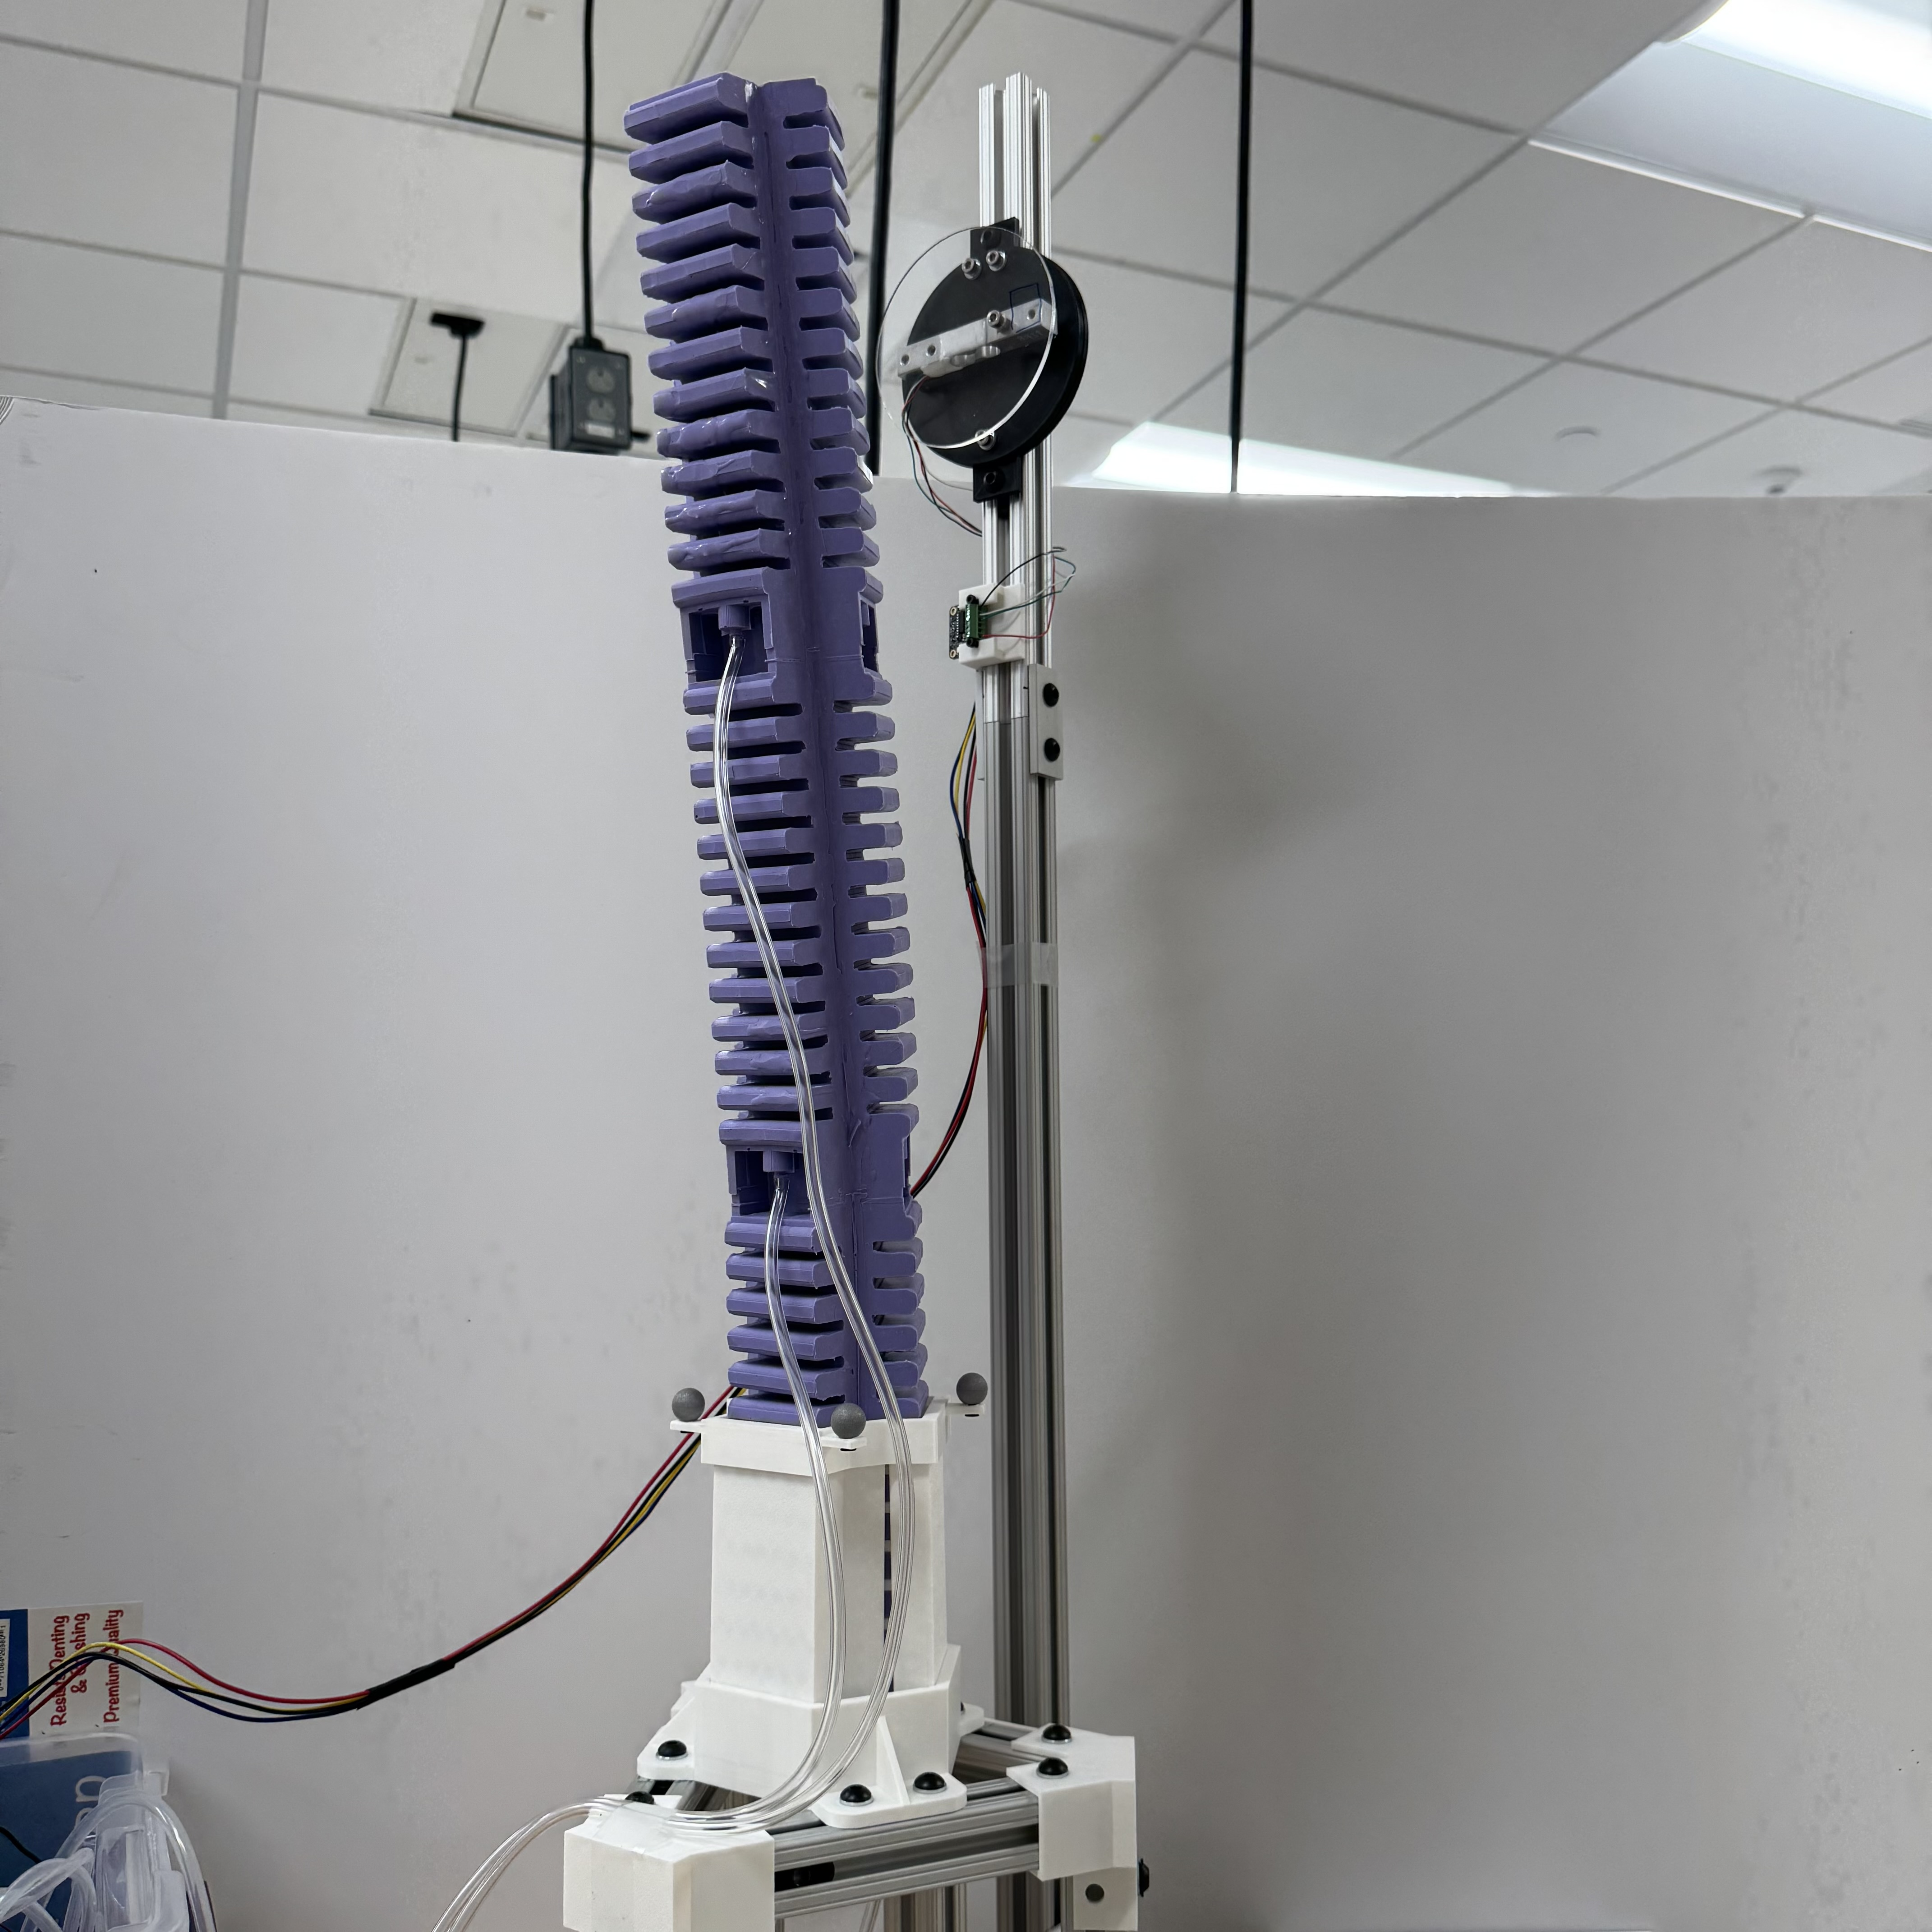
\includegraphics[width=0.6\textwidth]{graphics/limb.jpg}
    \caption{The 3-D pneumatically-actuated "limb" serving as our test bench platform}
    \label{soroimg}
\end{figure}

From the construction and physical characteristics of the robot alone, some semblance of what the dynamical terms and matrices of the robot are can be extracted. This initial application of the model to our system can be considered the "un-tuned" model. It can then be tuned by motor-babbling (passing in a series of randomized inputs--"babbles") our soft robot, simulate motor-babbling the soft robot \textit{using} the model, and then comparing the outputs between the two. Generally speaking, a "perfect" model would simulate an exact replica of the output that the robot itself physically produced. While the tuned model cannot do the same, it should simulate sufficiently accurate outputs when operating in configurations found within the boundaries established by the model's assumptions.

\begin{comment}
    \begin{figure}[!ht]
        \begin{subfigure}{0.3\textwidth}
            \subcaption{}
        \end{subfigure}
        \begin{subfigure}{0.3\textwidth}
            \subcaption{}
        \end{subfigure}
        \begin{subfigure}{0.3\textwidth}
            \subcaption{}
        \end{subfigure}
        \caption{An illustration comparing how the motor-babbling outputs would be simulated by a) the un-tuned model, b) a "perfect" model, and c) the tuned model}
        \label{varoutputs}
    \end{figure}
\end{comment}

The main goal of this phase is to calibrate the dynamic model to such an extent that it can sufficiently represent how the system \textit{responds} to an input signal. Since our soft robot is \textit{pneumatically}-actuated, that means the input signal will be in terms of pressure change. Roughly speaking, we want to ensure that for a given pressure change, the model simulates a change in configuration reflective of the change in configuration physically exhibited by the robot.   
%----------| 3. Control development, implementation, and validation
\subsection{Controller Implementation}
The third and final phase is meant to be the bulk of the \textit{experimental} work to be done. The phase will be initiated by first formulating the controller using known theories and current literature. This will consume the majority of the phase, as some amount of research into the body of literature available regarding controller design for the chosen model specifically will need to be done. Any reviews of theories or concepts deemed necessary at this point will also need to be conducted. The main functionality to be pursued for this controller is task-space regulation, and then trajectory tracking. A controller that can actuate the end effector of the robot around a point or bring it to trace a trajectory is necessary before physical compliance and environmental interaction can be explored.

\begin{figure}[!ht]
    \centering
    \includegraphics[width=0.6\textwidth]{graphics/trajDiag.PNG}
    \caption{The soft robot stabilizing around a trajectory}
    \label{taskspace}
\end{figure}

As the controller takes shape, simulations will then be run by implementing the controller onto the dynamic model. At this point, we are interested in seeing how closely does the output of the system come to the desired/reference configuration $\mathbf{r}$ when using the input signal $\mathbf{u}=f(\mathbf{x,r,e,t,...})$ produced by the controller. The big focus of this proposed thesis remains hardware implementation, but this phase includes a simulation step essentially as a validation method. The simulations should point out any glaring limitations or discrepancies in the controller formulated. 

Finally, the controller can then be implemented on our soft robot. In this final step, any major or fundamental changes to the controller would ideally be avoided. The main goal of the experimentation to be conducted on the hardware is really to serve as an assessment of the controller formulation: how well does the methodology used to formulate the controller stand up to physical implementation? While results that inform us to change certain tuning or calibration parameters can be readily implemented, the deeper and more meaningful insights around controller design methodology for this scenario shall be left for future work.